前章で記したとおり、信号伝送方式にはベースバンド伝送とブロードバンド伝送がある。ベースバンド伝送は信号そのものに応じて電圧を変化させて送る方式であった。ブロードバンド伝送ではキャリア(搬送波)にデータを乗せて信号を送る。この章ではまず、キャリアにデータを乗せる手法である\textbf{変調}\index{へんちょう@変調}(modulation)と、キャリアに乗っているデータを取り出す\textbf{復調}\index{ふくちょう@復調}(demodulation)について解説する。次いで、キャリアを複数同時に伝送する方法である多重化について記す。

\section{変調}

帯域伝送においては、キャリアを一つ用意しこれを変化させることでデータを乗せる。つまり、標準的な波(データが乗っていないキャリア単体)からの差分となる部分にデータを乗せるわけである。変調とはキャリアの要素(振幅・周波数・位相)のいずれかをデータに応じて変化させることであり、復調とは逆にキャリアとの差分からデータを取得することである。ベースバンド伝送での電圧の変化方式が複数あったのと同様、キャリアのどの要素を変化させるかによって複数の変調方式がある。

\subsubsection{【補足】波の要素}

\begin{center}
\begin{minipage}[]{0.75\linewidth}
\begin{screen}
\begin{center}
本節は前提知識の補足である。\\
既知の読者におかれては飛ばして次節を読まれたい。
\end{center}
\end{screen}
\end{minipage}
\end{center}

先に、キャリアの要素を振幅・周波数・位相と書いたが、波の要素について補足説明しておく。波の式$w(t)$は、三角関数を用いて以下のように記される(ここでは$\sin$を用いたが、$\cos$を用いても同様である)。
\begin{equation}
w(t)=A\sin (2\pi ft+\theta_0)
\end{equation}
この時、$A$を波の振幅(Amplitude)、$f$を周波数(frequency)、$\theta_0$を位相(phase)と呼ぶ。物理的な意味付としては、振幅:波の最大の振れ幅を示す値、周波数:単位時間あたりに何周期の波が入るか、位相:$t=0$における波の振れがどの程度進んでいるか、ということになる。図\ref{fig6_1}にそれぞれを図解する。

\begin{figure}[htbp]
\centering
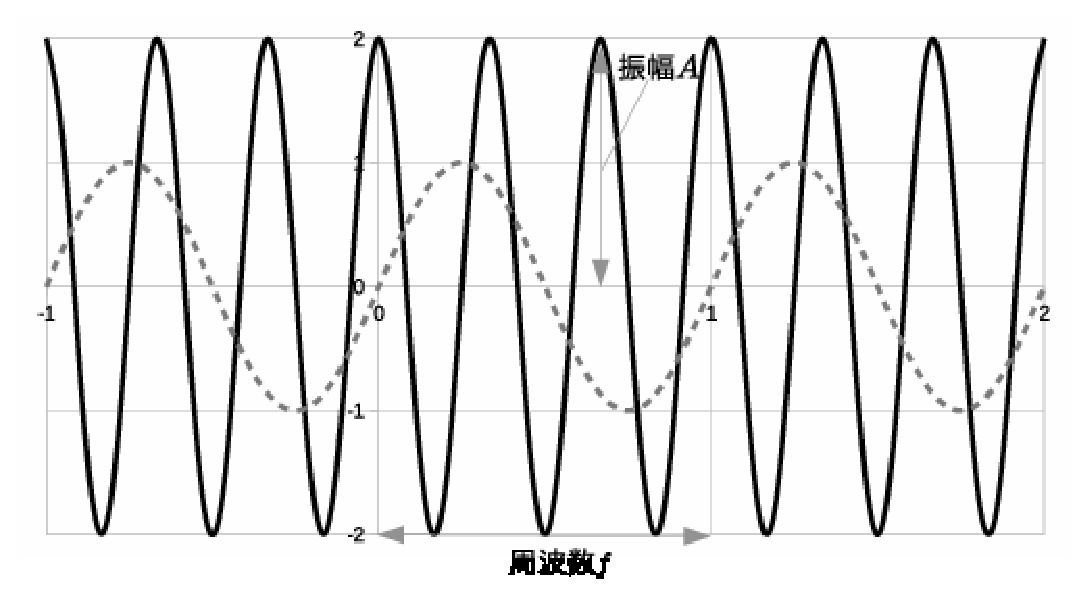
\includegraphics[width=0.9\linewidth,keepaspectratio]{fig/fig6_1.eps}
\caption{波$w_1(t)=\sin 2\pi t$(破線)と波$w_2(t)=2\sin (6\pi t+\frac{\pi}{2})$(実線)の様子。振幅$A=2$と周波数$f=3$を記載。}
\label{fig6_1}
\end{figure}

図\ref{fig6_1}においては、破線により波$w_1(t)=\sin 2\pi t$という位相0、振幅・周波数1という単純な波を示している。また、実線で波$w_2(t)=2\sin (6\pi t+\frac{\pi}{2})$が書かれてあるが、その振れ幅が2倍になっていること、つまり振幅が二ということがわかるであろう。また、周波数についても、0から1の間に、破線の方は1周期の波が入っているのに対し、実線の方は3周期の波が入っている。位相については図の中に書き込めていないが、$w_2(t)$は$t=0$においてちょうど最大振幅まで振れた時、つまり$\frac{\pi}{2}$だけ進んだ時となっている。

このように、振幅・周波数・位相により波の様態は変化する。以降の説明では、これら3要素をどのように変化させるのかを見ていくこととなる。

\subsubsection{【補遺】変調の原理}
\begin{center}
\begin{minipage}[]{0.75\linewidth}
\begin{screen}
\begin{center}
本節は大筋に影響しない。\\
難解あるいは興味索然たるものと感じる折には\\
飛ばして次節を読まれたい。
\end{center}
\end{screen}
\end{minipage}
\end{center}

変調について概念的な説明を行ったが、実現するために数式に落とし込んだ原理を説明しておこう。

出発点はFourier展開の係数の式(\ref{eq_2_2})である。
\begin{equation}
a_k=\int^{L}_{-L} f(x) \cos f_kx dx \quad , \quad b_k=\int^{L}_{-L} f(x) \sin f_kx dx \tag{\ref{eq_2_2}}
\end{equation}

元の信号$f(x)$とキャリア$\cos \omega_c x$の積を取り、このFourier展開を考える。式(\ref{eq_2_2})の$f(x)$を$f(x)\cos \omega_c x$に置き換え、三角関数の積を和に直せば
\begin{equation}
a_k=\frac{1}{2}\int^{L}_{-L} f(x) \left(\cos (\omega_c-f_k) x + \cos (\omega_c+f_k) x \right)dx \label{eq_6_1}
\end{equation}
となる。($b_k$についても、$\cos$を$\sin$に変えた形式で同じである。)キャリアとの積を取った結果、係数における三角関数が上記のように$\pm f_k$だけ変化する。これは、換言すればキャリアの周波数が$\pm f_k$だけ推移したものになる。この推移によってキャリアに信号が乗っているか否か区別でき、またその差異から信号を取り出すことができるのである。

なお、先の推移のうち、正の側を上側波帯、負の側を下側波帯と呼ぶ。信号を取り出すためには一方があれば十分であるため、片方だけを利用するSSB単側波帯通信方式なども実用化されている。

\subsection{振幅変調}

波の3要素のうち、振幅を変えることでデータを乗せる方法を\textbf{振幅変調}\index{しんぷくへんちょう@振幅変調}(Amplitude Modulation,\textbf{AM}\index{AM|see{振幅変調}})と呼ぶ。ラジオにおける中波放送(いわゆるAMラジオ)や短波放送がこの振幅変調により信号を送っている。

送るべき信号の周波数帯に比べて、十分に大きい周波数をもつキャリアを用意する。すると、信号の縮尺でみた時、キャリアはほぼ長方形に塗りつぶしたようなグラフとなる。このキャリアの振幅を信号に応じて変調する(図\ref{fig6_2})。変調後の波は軸の上下両方に信号が乗っていることがわかる。

\begin{figure}[htb]
\centering
\includegraphics[width=0.6\linewidth,keepaspectratio,bb=0 0 489 245]{fig/fig6_2.png}
\caption{振幅変調のグラフ。Asunaro-net(アスナロネット)より引用}\label{fig6_2}
\end{figure}

同じことを式で示す。伝送する信号(原信号)として正弦波$f(t)=A_s\cos\omega_st$、キャリアとして$f_c(t)=A_c\cos(\omega_ct+\theta_c)$を想定すると(但し、キャリアの仮定から$\omega_s\ll\omega_c$)、振幅変調によりキャリアは振幅項$A_c$が$A_c+f(t)$に置き換わり、全体として次のように表せる。
\begin{eqnarray}
f_c(t)&=&(A_c+A_s\cos\omega_st)\cos(\omega_ct+\theta_c) \nonumber \\
&=&A_c\left(1+\frac{A_s}{A_c}\cos\omega_s t\right)\cos(\omega_ct+\theta_c) \label{eq_6_2}
\end{eqnarray}
ここで$m=A_s/A_c$(図\ref{fig6_2}の$P,Q$を用いると$m=(P-Q)/(P+Q)$とも表せる)は\textbf{変調度}\index{へんちょうど@変調度}(modulation degree)と呼ばれ、変調の深さの程度を表す。変調度の値が大きいほど信号波の振幅が大きくなりクリアになる。ただし100\%を超える状態(過変調)となると、復調信号の波形が歪み、また不要波を発生して他の通信に妨害を与えてしまうので、放送では変調度の最大値が厳しく規定されている。

これによって届いた信号の上半分(半波整流という方法で得られる)の包絡線をとり、直流除去することで復調を実現できる。包絡線を取る手段には、コンデンサの充放電を利用して包絡線を再現する包絡線検波器が一般的である。また、ハイカットフィルター(高周波数成分を除去する)をかけることで包絡線を取ることもできる。

なお、ディジタルデータの伝送ではASK(Amplitude Shift Keying)又はOOK(On Off Keying)とも呼ばれ、0に対しては無変調、1に対しては変調という取扱をすることが多い。伝送路で発生する雑音やレベル変動に弱いものの、非常に安価な回路で実現できること、伝送帯域を有効利用できること、非同期信号の伝送が可能であることといった利点を有する。

\subsubsection{【補遺】振幅変調における周波数推移の例}
\begin{center}
\begin{minipage}[]{0.75\linewidth}
\begin{screen}
\begin{center}
本節は大筋に影響しない。\\
難解あるいは興味索然たるものと感じる折には\\
飛ばして次節を読まれたい。
\end{center}
\end{screen}
\end{minipage}
\end{center}

キャリアの周波数推移が変調の原理であることは既に述べた。ここでは、振幅変調で実際に周波数推移を見てみよう。

式(\ref{eq_6_2})は次のように展開できる。
\begin{eqnarray}
f_c(t)&=&A_c\cos(\omega_ct+\theta_c)+A_cm\cos\omega_st\cdot\cos(\omega_ct+\theta_c) \nonumber \\
&=&A_c\cos(\omega_ct+\theta_c)\nonumber \\
&\ &\quad +\frac{A_cm}{2}\left[\cos\{(\omega_c-\omega_s)t+\theta_c\}+\cos\{(\omega_c+\omega_s)t+\theta_c\}\right] \label{eq_6_3}
\end{eqnarray}

これより振幅変調の結果、周波数領域では$\omega_c$とそれより$\pm\omega_s$だけ離れた成分、$-\omega_c$とそれより$\pm\omega_s$だけ離れた成分が発生していることがわかる。

\subsection{周波数変調}
信号の強度に応じて、キャリアの周波数を変える変調方式を\textbf{周波数変調}\index{しゅうはすうへんちょう@周波数変調}(Frequency Modulation,\textbf{FM}\index{FM|see{周波数変調}})と呼ぶ。デジタル伝送の場合はFSK(Frequency Shift Keying)とも呼ばれる。FNラジオやアマチュア無線などで広く利用される。

送るべき信号の周波数帯に比べて、十分に大きい周波数をもつキャリアを用意する。ここまでは振幅変調と同様である。この時、信号の強度に応じて周波数を変化させる(図\ref{fig6_3})。

\begin{figure}[htb]
\centering
\includegraphics[width=0.8\linewidth,keepaspectratio,bb=0 0 422 307]{fig/fig6_3.jpg}
\caption{周波数変調のグラフ。EDN Japan 「これだけは知っておきたいアナログ用語:FM変調」より引用}\label{fig6_3}
\end{figure}

ただし、そのまま周波数を変更すると復調の際に問題がおこるため、実際には信号の積分を位相に付け加える。伝送する信号(原信号)として正弦波$f(t)=A_s\cos\omega_st$、キャリアとして$f_c(t)=A_c\cos(\omega_ct)$を想定するとき(簡単のため、位相項を省いている)、キャリアの許容する最大の周波数変化を$\delta \omega$として
\begin{equation}
f_c(t) = A_c \cos\left(\omega_c t+\frac{\delta \omega}{\omega_s}\sin\omega_s t\right) \label{eq_6_4}
\end{equation}
とするのが周波数変調である。なお、$m=\delta \omega/\omega_s$が周波数変調における変調度である。これが大きいほど専有帯域が広くなってしまうが、S/N比が向上する。復調の際には、搬送波を微分回路などに通して微分した後、整流・直流カットすることで信号を取り出す。

周波数変調の利点は、振幅が一定であることからノイズに強いということである。振幅方向のノイズは振幅制限器により容易に取り除け、先に書いたように変調度の調整でS/N比の向上も可能である。また、弱肉強食特性と呼ばれる特性があり、弱い信号が混信したとしても先の振幅制限機の都合取り除かれる。これは、混信防止の観点では役に立つが、より強い通信により遮られうるということでもある。

\subsection{位相変調}
\textbf{位相変調}\index{いそうへんちょう@位相変調}(Phase Modulation,\textbf{PM}\index{PM|see{位相変調}})とは、キャリアの位相を変える変調方式であるが、先の周波数変調でも周波数とは言い条、実のところ位相を変更していた。つまり、周波数変調と位相変調は本質的に同じものとなる。しかし、これはアナログの場合の話であり、デジタルデータの伝送、PSK(Phase Shift Keying)の場合にはまた異なる様相を呈する。

デジタル伝送における振幅変調、周波数変調、位相変調(つまりASK,FSK,PSK)の概念を図\ref{fig6_4}に示す。
\begin{figure}[htb]
\centering
\includegraphics[width=0.8\linewidth,keepaspectratio,bb=0 0 616 472]{fig/fig6_4.png}
\caption{デジタル変調の概念図。宮崎技術研究所サイトより引用}\label{fig6_4}
\end{figure}

ASK,FSKは各々AM,FMを0,1に対応させたということで理解できるであろう。しかし、PSKの場合、FSKとはまるきり異なり、0の波形と1の波形の位相がちょうど180度変わっている。つまり、アナログな伝送においては周波数変調が復調の都合から結果的に位相に頼っている所、デジタル変調ではその事情が変わるゆえに位相変調と周波数変調がはっきりと分かれるのである。

デジタル変調における位相変調には幾つかの手法があるが、ここではBPSKとQPSKを紹介する。

\subsubsection{BPSK}

位相変調の最も基本的なものが、Binary PSK,\textbf{BPSK}\index{BPSK}である。この方式では、ある位相の波とちょうど180度違う波とをそれぞれ0/1に対応させる(図\ref{fig6_5})。これは、二元値となるため雑音に強いという長所がある。特に伝送路の状態に応じて適切な通信速度に変えていくようなプロトコルを用いる場合は、初期のデータリンクを確立させるフェーズでは、このBPSKで通信を開始することが多い。

\begin{figure}[htb]
\centering
\includegraphics[width=0.9\linewidth,keepaspectratio,bb=0 0 588 524]{fig/fig6_5.jpg}
\caption{BPSKの概念図。ASCII.jp「きっちり知りたい無線LANの変調技術の基礎」より引用}\label{fig6_5}
\end{figure}

\subsubsection{QPSK}

BPSKでは180度違う位相により0と1を表したが、今度は90度ずつ違う4つの位相を用いることにしよう。すると、この結果として4値=00,01,10,11を表すことができる。この手法がQuadrature PSK,\textbf{QPSK}\index{QPSK}である(図\ref{fig6_6})。BPSKと同じ搬送波を用いていても、表すデータ量が2倍に増えているので2倍の伝送速度となる。この手法は、携帯電話の通信で使われる。他、Wi-fi等を定めたIEEE802.11シリーズでは直前の状態との差分データをこの手法により伝送するDQPSK(Differential QPSK)が使われている。

\begin{figure}[htb]
\centering
\includegraphics[width=0.8\linewidth,keepaspectratio,bb=0 0 588 575]{fig/fig6_6.jpg}
\caption{QPSKの概念図。ASCII.jp「きっちり知りたい無線LANの変調技術の基礎」より引用}\label{fig6_6}
\end{figure}

しかし、2値を4値にして位相にしたということは、誤差として許容できる位相のズレが半分になったということである。したがって、当然にBPSKよりは雑音に弱くなっている。

これと同じ考えを用いて、8位相を使い3bitを送るものに8PSKがある。更に細かくしていけば16PSKや32PSKなども考えられるが、雑音の影響などから実用的に使われているのは8PSKぐらいまでである。

\subsubsection{変調速度}

デジタル変調では、図\ref{fig6_4}の例からわかるようにキャリアの何周期かに対してデータを対応させて伝送するのが普通である。言い換えれば、キャリアの何周期かを用いて1回の変調を行うということである。キャリアは1秒あたりに$f_c$(周波数)回の周期を持つから、結局1秒あたりに何度の変調を行うかがわかる。このようにして求められる1秒間の変調回数を\textbf{変調速度}\index{へんちょうそくど@変調速度}と呼ぶ。通常、1秒間の変調回数はBaud(ボー)という単位で表す。

昔のモデムなどには、その速度の指標として変調速度が記述されていた。一方、インターネットの普及以後は、伝送速度にはbps(bit per second)が使われる。これらの変換は容易である。1回の変調により何bitのデータとなるのかが分かれば、変調速度に1回あたりのデータ長をかけることでbpsに変換できる。BPSK方式であれば1baud=1bpsであるし、QPSK方式であれば1baud=2bpsである。

\subsection{変調方法の組み合わせ:QAM}
ここまでに紹介した位相変調と振幅変調を組み合わせることで、より速くデータを送ることができる。そのうち、比較的単純な例である\textbf{直交振幅変調}\index{ちょっこうしんぷくへんちょう@直交振幅変調}(quadrature amplitude modulation,\textbf{QAM}\index{QAM|see{直交振幅変調}})を紹介しよう。

QAMでは、QPSKのように位相に複数値を与えるだけでなく、振幅方向にも複数値を与える。例えば振幅を4段階、QPSKと同様に位相を4段階とすると、16値=4bitが一度の変調で送れることとなる(この場合16QAMと呼ぶ)。一方、振幅変調が入ったことにより振幅方向の雑音にも弱くなっている。速さとのトレードオフと言える。

スマートフォン等で無線通信の利用が確実に増えている中にあるため、無線通信の高速化は今も日々進められている。現代では4096値(単純には12bit)の変調ができる4096QAMのような手法も考案されている。Wi-fiの標準規格であるIEEE 802.11では、64QAMや256QAMが採用されている。

\subsection{パルス符号変調(PCM)}
ここまで扱ってきた変調は、基本的にはアナログのデータ・デジタルのデータをそのまま変調する方法である。ところが、ここまでに見てきたようにアナログデータはデジタルデータ化して保存できる(標本化・量子化・符号化)。この変換と変調を同時に行うのが\textbf{パルス符号変調}\index{ぱるすふごうへんちょう@パルス符号変調}(Pulse Code Modulation,\textbf{PCM}\index{PCM|see{パルス符号変調}}である。符号を表す方法は、先の各デジタル変調と変わらないが、PCMの特徴として、元のデータをそのまま並べるリニアPCMや、前のデータとの差分を並べるDPCMといった、データの並べ方に関する手法の差異がある。

いわゆるデジタル音源の変調は、この方式である。音楽CDの規格であるCD-Aではサンプリング周波数44.1kHz、量子化ビット数16bit、2chステレオのPCMによる。

\section{多重化}
変調された波を送る際、通常、キャリア毎に一本の伝送路を用意するのではなく、複数のキャリアで一本の伝送路を共有利用する。これを\textbf{多重化}\index{たじゅうか@多重化}という。多重化により、複数からの通信を一度に受けられる、伝送路をまとめることで整備のコストダウンにつながるなどのメリットが得られる。

\subsection{周波数分割多重化}
ラジオを受信する際には、通常、受信する周波数を定め、他の周波数を受け取らない。といっても、周波数により自動的に電波発信源を選ぶようなことをしているわけではなく、ラジオの電波がすべて合わさったものから、特定の周波数を取り出しているのである。このように、周波数の異なるキャリアを、互いに干渉しないように定めて多重化する方法を\textbf{周波数分割多重化}\index{しゅうはすうぶんかつたじゅうか@周波数分割多重化}(Frequency Division Multiplex,\index{FDM})と呼ぶ。

十分大きな周波数を持つキャリアに対して、変調波はキャリアの元の周波数を基準に多少増減した範囲の周波数に収まる。そこで、各キャリアに対して変調後の周波数の範囲を設け、これを周波数単位で取り出せば(取り出すのはフィルタを用いることで実現できる)、必要となる変調波だけを取り出すことができる。

なお、周波数を変化させるということは、言い換えれば波長を変化するということでもある。波長による多重化として実装する場合は\textbf{波長分割多重化}\index{はちょうぶんかつたじゅうか@波長分割多重化}(Wavelength Division Multiplex,\textbf{WDM}\index{WDM|see{波長分割多重化}})と呼ぶ。特に光ファイバにおいては(その性質上)波長で考えた方が都合が良いため、WDMあるいは光波長多重通信と呼び、異なる波長の光を統合して送信している。周波数分割多重化と波長分割多重化は、その本質的な部分こそ同等であるが、取り扱う対象(特に、電気か光か)によって性質や実装に多少の差異がある。

\subsection{時分割多重化}
\textbf{時分割多重化}\index{じぶんかつたじゅうか@時分割多重化}(Time Division Multiplex,\index{TDM})は主にデジタル通信で使われる方法で、パルス列の合間に別のチャネルの信号を挿入する方法による多重化である。現代のコンピュータのマルチタスクなどとも同等の考えであるが、ごく短い周期で送るデータを変更することで多重化しているように見せるということである。

時分割多重化では、データAのある一定数の符号とデータBのある一定数の符号とを交互に送信する。通常、データAの送信には隙間があるはずで、その隙間を縫うようにデータBを入れていくのである。これにより、通常の2倍の量のデータを送信することができる(もちろん、入れるチャンネルを増やせばそれだけ速くなる。)

\subsection{符号分割多重化}
\textbf{符号分割多重化}\index{ふごうぶんかつたじゅうか@符号分割多重化}(Code Division Multiple,\textbf{CDM}\index{CDM|see{符号分割多重化}})は、符号分割多重接続(\textbf{CDMA}\index{CDMA|see{符号分割多重化}})とも呼ばれ、第3世代携帯電話(3G通信)などの通信方式に使われている多重化方式である。

ここまでに紹介した方式と違い、符号分割多重化方式では周波数の同じ信号を複数同時に送信する。このとき、必要な信号以外の信号は、全てノイズといえる。そこで、必要な信号だけを取り出せるような「鍵」となる符号を用意しておき、その符号によってエンコード・デコードすることでデータを送受信する。より簡単に言えば、全ての送るデータにそれとわかるようなフラグを立てておき、特定のフラグのものだけを取り出す、ということである。
\subsection{空間分割多重化}
上記のような様々な方法によりまとめて送信することで効率よくデータを送ることができるようになるわけだが、これらで間に合わない場合であっても、最終的には単に接続路を増やすことでも多重化が可能であり、これを\textbf{空間分割多重化}\index{くうかんぶんかつたじゅうか@空間分割多重化}(Space Division Multiplex,\textbf{SDM}\index{SDM|see{空間分割多重化}})。コストダウンよりは性能向上への解決策である。


\section*{演習問題}
\begin{problems}
\item 一般に、AMラジオよりもFMラジオの方がクリアな音声になると言われる。この理由を説明しなさい。

\item ADSLモデムでは、音声通話で利用しない周波数帯域で複数の搬送波を使ってデータ通信を行います。搬送波の数が200であり、各搬送波について1変調あたり128値、変調速度1000ボーであったとすると、伝送速度は何Mbpsになるか求めなさい。

\item 自身に馴染みのあるWi-fiルータについて、その変調方式を調べてみなさい。(例えば、筆者が使っているTP-Link社のArcher C3150という機種は1024QAMを採用している。)

\item ラジオの周波数を合わせる際、周波数が多少ずれていても音声が聞こえる。この理由を説明しなさい。
\end{problems}
